\chapter{Sprachaufnahme: Sprechen erfassen und sichtbar machen} 

Gesprochene Sprache ist flüchtig. Um die Transmission von Sprachschall zwischen Schallquelle (z.\thinspace B. Sprecher*in) und Schallsenke (z.\thinspace B. Hörer*in) genau untersuchen zu können (also nicht mittels synchroner Transkription), muss der Sprachschall durch eine Sprachaufnahme festgehalten werden (vgl. auch Kapitel Sprachdatenbanken). 

\section{Stichworte zur Vorlesung \em{Sprachakustik}}

Schall, Schwingung, akustische Signaltypen, (Grund-)Frequenz, Formanten, Oszillogramm, Spektrum, Spektrogramm, Quelle-Filter... $\rightarrow$ {\tt L3\underline{\ }Akustik.pdf}
\begin{figure}[htbp]
\begin{center}
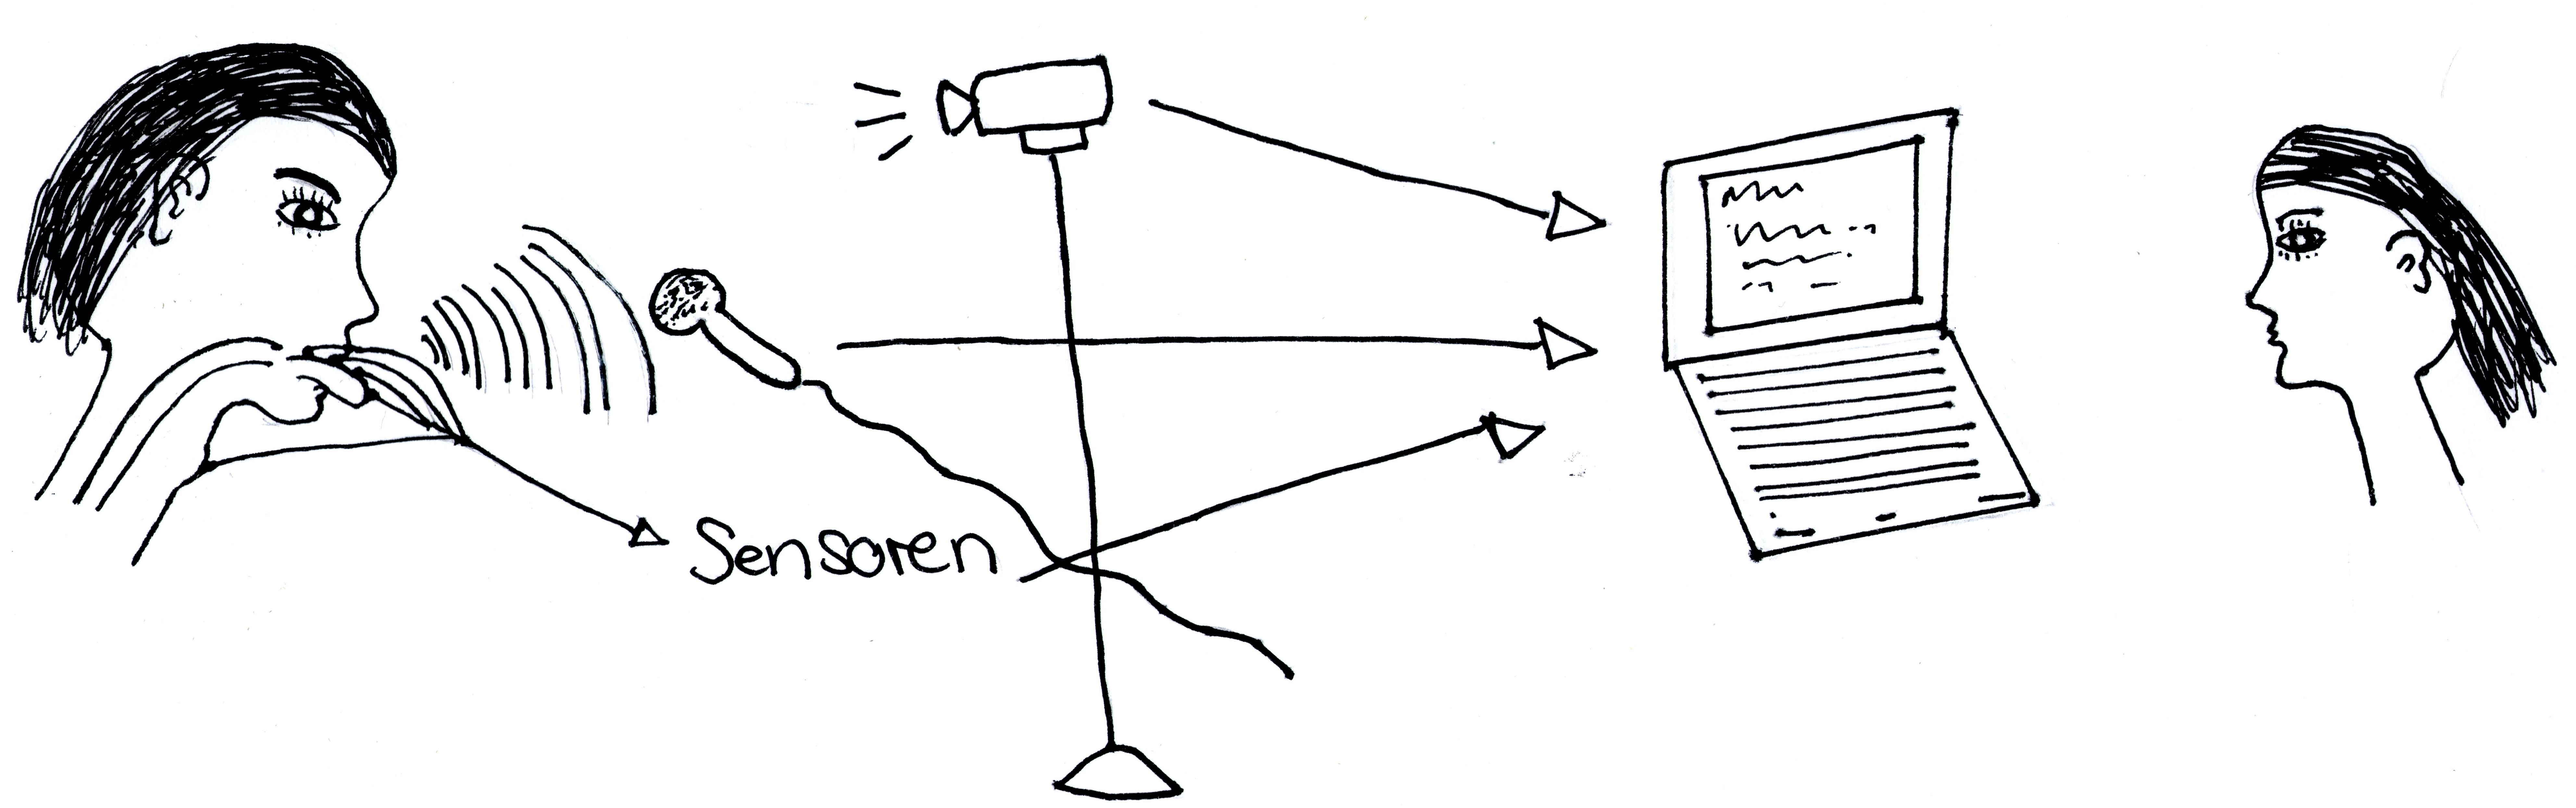
\includegraphics[width=\textwidth]{grafiken/sprachaufnahme/sprechen-erfassen.jpg}
\label{t2}
\end{center}
\end{figure}

\section{Übungen}

\subsection*{Aufnahmeübung}


Die Sprachaufnahme erfolgt in Kleingruppen an den mitgebrachten Laptops. Jede Gruppe erhält einen schriftlichen Arbeitsauftrag und ggf. ein Mikrofon oder Aufnahmegerät. Führen Sie die Aufnahme wie angegeben durch und sichern Sie die Audiodateien. In der nächsten Stunde werden wir auf die Dateien zurückgreifen.
\vspace*{7cm} 

Tipp: \newline \\ 

\begin {minipage} {0.1\textwidth}

\includegraphics[width=\textwidth]{grafiken/sprachaufnahme/praat.png}
\end{minipage}
\hspace {1cm}
\begin{minipage} {0.7\textwidth}
Praat können Sie kostenlos unter {\tt www.fon.hum.uva.nl/praat/} (Stand: 12.10.2018) herunterladen. 
\end {minipage}


\begin {minipage} {0.1\textwidth}
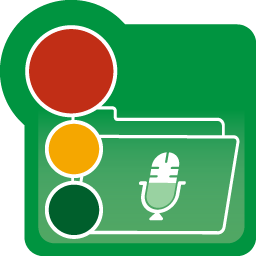
\includegraphics[width=\textwidth]{grafiken/sprachaufnahme/speechrecorder.png}
\end{minipage}
\hspace{1cm}
\begin{minipage} {0.6\textwidth}
Ebenfalls kostenlos herunterladen können Sie verschiedene Aufnahmeprogramme, die sich für phonetische Zwecke eignen, darunter SpeechRecorder ({\tt www.speechrecorder.org}), Audacity  ({\tt www.audacityteam.org}) und Praat (siehe oben) (Links Stand: 12.10.2018).
\end {minipage}



\begin{figure}[htb]
\begin{center}
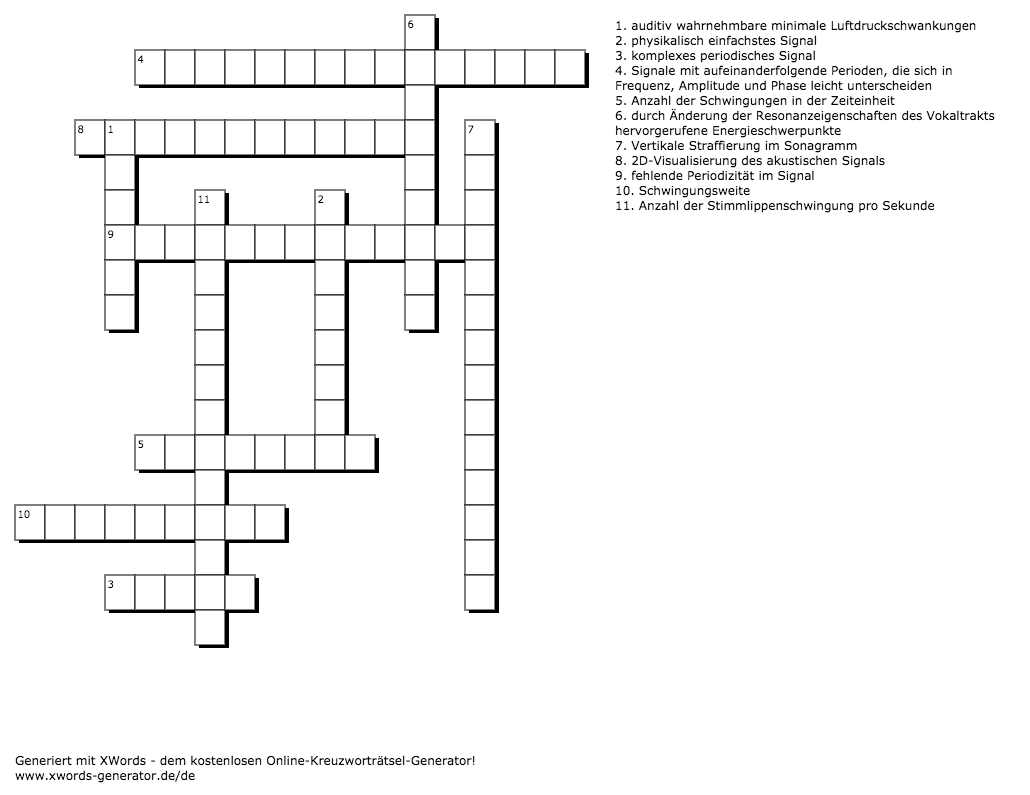
\includegraphics[width=1.2\textwidth]{grafiken/sprechen/kreuzwortraetsel.png}
\caption{Kreuzworträtsel}
\label{fig5}
\end{center}
\end{figure}
